% (find-LATEX "2021-1-C2-P2.tex")
% (defun c () (interactive) (find-LATEXsh "lualatex -record 2021-1-C2-P2.tex" :end))
% (defun C () (interactive) (find-LATEXsh "lualatex 2021-1-C2-P2.tex" "Success!!!"))
% (defun D () (interactive) (find-pdf-page      "~/LATEX/2021-1-C2-P2.pdf"))
% (defun d () (interactive) (find-pdftools-page "~/LATEX/2021-1-C2-P2.pdf"))
% (defun e () (interactive) (find-LATEX "2021-1-C2-P2.tex"))
% (defun o () (interactive) (find-LATEX "2021-1-C2-P2.tex"))
% (defun u () (interactive) (find-latex-upload-links "2021-1-C2-P2"))
% (defun v () (interactive) (find-2a '(e) '(d)))
% (defun d0 () (interactive) (find-ebuffer "2021-1-C2-P2.pdf"))
% (defun cv () (interactive) (C) (ee-kill-this-buffer) (v) (g))
%          (code-eec-LATEX "2021-1-C2-P2")
% (find-pdf-page   "~/LATEX/2021-1-C2-P2.pdf")
% (find-sh0 "cp -v  ~/LATEX/2021-1-C2-P2.pdf /tmp/")
% (find-sh0 "cp -v  ~/LATEX/2021-1-C2-P2.pdf /tmp/pen/")
%     (find-xournalpp "/tmp/2021-1-C2-P2.pdf")
%   file:///home/edrx/LATEX/2021-1-C2-P2.pdf
%               file:///tmp/2021-1-C2-P2.pdf
%           file:///tmp/pen/2021-1-C2-P2.pdf
% http://angg.twu.net/LATEX/2021-1-C2-P2.pdf
% (find-LATEX "2019.mk")
% (find-CN-aula-links "2021-1-C2-P2" "2" "c2m211p2" "c2p2")
%
% Video (not yet):
% (find-ssr-links "c2m211p2" "2021-1-C2-P2")
% (code-video     "c2m211p2video" "$S/http/angg.twu.net/eev-videos/2021-1-C2-P2.mp4")
% (find-c2m211p2video "0:00")

% «.defs»		(to "defs")
% «.defs-T-and-B»	(to "defs-T-and-B")
% «.title»		(to "title")
% «.regras-e-dicas»	(to "regras-e-dicas")
% «.vamos-usar»		(to "vamos-usar")
% «.questao-1»		(to "questao-1")
% «.questao-1-cont»	(to "questao-1-cont")
% «.questao-2»		(to "questao-2")
% «.questao-2-cont»	(to "questao-2-cont")
% «.gabarito»		(to "gabarito")
% «.questao-1a-gab»	(to "questao-1a-gab")
% «.questoes-1bc-gab»	(to "questoes-1bc-gab")
% «.questoes-1def-gab»	(to "questoes-1def-gab")
% «.questoes-2ab-gab»	(to "questoes-2ab-gab")
% «.questoes-2cd-gab»	(to "questoes-2cd-gab")
% «.questao-2e-gab»	(to "questao-2e-gab")
% «.questoes-2fg-gab»	(to "questoes-2fg-gab")
%
% «.djvuize»		(to "djvuize")

\documentclass[oneside,12pt]{article}
\usepackage[colorlinks,citecolor=DarkRed,urlcolor=DarkRed]{hyperref} % (find-es "tex" "hyperref")
\usepackage{amsmath}
\usepackage{amsfonts}
\usepackage{amssymb}
\usepackage{pict2e}
\usepackage[x11names,svgnames]{xcolor} % (find-es "tex" "xcolor")
\usepackage{colorweb}                  % (find-es "tex" "colorweb")
%\usepackage{tikz}
%
% (find-dn6 "preamble6.lua" "preamble0")
%\usepackage{proof}   % For derivation trees ("%:" lines)
%\input diagxy        % For 2D diagrams ("%D" lines)
%\xyoption{curve}     % For the ".curve=" feature in 2D diagrams
%
\usepackage{edrx21}               % (find-LATEX "edrx21.sty")
\input edrxaccents.tex            % (find-LATEX "edrxaccents.tex")
\input edrx21chars.tex            % (find-LATEX "edrx21chars.tex")
\input edrxheadfoot.tex           % (find-LATEX "edrxheadfoot.tex")
\input edrxgac2.tex               % (find-LATEX "edrxgac2.tex")
%
%\usepackage[backend=biber,
%   style=alphabetic]{biblatex}            % (find-es "tex" "biber")
%\addbibresource{catsem-slides.bib}        % (find-LATEX "catsem-slides.bib")
%
% (find-es "tex" "geometry")
\usepackage[a6paper, landscape,
            top=1.5cm, bottom=.25cm, left=1cm, right=1cm, includefoot
           ]{geometry}
%
\begin{document}

%\catcode`\^^J=10
%\directlua{dofile "dednat6load.lua"}  % (find-LATEX "dednat6load.lua")

% %L dofile "edrxtikz.lua"  -- (find-LATEX "edrxtikz.lua")
% %L dofile "edrxpict.lua"  -- (find-LATEX "edrxpict.lua")
% \pu

% «defs»  (to ".defs")
% (find-LATEX "edrx15.sty" "colors-2019")
%\long\def\ColorRed   #1{{\color{Red1}#1}}
%\long\def\ColorViolet#1{{\color{MagentaVioletLight}#1}}
%\long\def\ColorViolet#1{{\color{Violet!50!black}#1}}
%\long\def\ColorGreen #1{{\color{SpringDarkHard}#1}}
%\long\def\ColorGreen #1{{\color{SpringGreenDark}#1}}
%\long\def\ColorGreen #1{{\color{SpringGreen4}#1}}
%\long\def\ColorGray  #1{{\color{GrayLight}#1}}
%\long\def\ColorGray  #1{{\color{black!30!white}#1}}
%\long\def\ColorBrown #1{{\color{Brown}#1}}
%\long\def\ColorBrown #1{{\color{brown}#1}}
%\long\def\ColorOrange#1{{\color{orange}#1}}
%
%\long\def\ColorShort #1{{\color{SpringGreen4}#1}}
%\long\def\ColorLong  #1{{\color{Red1}#1}}
%
%\def\frown{\ensuremath{{=}{(}}}
%\def\True {\mathbf{V}}
%\def\False{\mathbf{F}}
%\def\D    {\displaystyle}

\def\frown{\ensuremath{{=}{(}}}
\def\True {\mathbf{V}}
\def\False{\mathbf{F}}
\def\D    {\displaystyle}

\def\Rd#1{\ColorRed{#1}}
\def\Rdq{{\Rd{?}}}
\def\eqq{\overset{\Rdq}{=}}     % equal with a question mark
\def\eqq{\overset{?}{=}}        % equal with a question mark
\def\eqvs#1#2{\ph{#1}\rotl{=}\ph{#2}} % vertical equal with spaces

\def\dydx{\frac{dy}{dx}}
\def\pfo #1{\ensuremath{\mathsf{[#1]}}}
\def\pfot#1{\ensuremath{\textsf{[#1]}}}

\def\EDOVSGone{
  \left(
  \begin{array}{rcl}
  \D \frac{dy}{dx} &=& \D \frac{f(x)}{g(y)} \\ [10pt]
        g(y) \, dy &=&   f(x) \, dx         \\ [5pt]
      ∫ g(y) \, dy &=& ∫ f(x) \, dx         \\
   \rotl{=}\ph{mm} & & \ph{mm}\rotl{=}      \\[-5pt]
        G(y) + C_1 & & F(x) + C_2           \\
                                               [5pt]
        G(y) + C_1 &=& F(x) + C_2           \\ [5pt]
        G(y)       &=& F(x) + C_2 - C_1     \\
                   &=& F(x) + C_3           \\
                                               [5pt]
      G^{-1}(G(y)) &=& G^{-1}(F(x) + C_3)   \\
   \rotl{=}\ph{mm} & &                      \\[-5pt]
          y\ph{mm} & &                      \\
  \end{array}
  \right)
  }

\def\EDOVSGtwo{
  \left(
  \begin{array}{rcl}
  \D \frac{dy}{dx} &=& \D \frac{f(x)}{g(y)} \\ [10pt]
                 y &=& G^{-1}(F(x) + C_3)   \\
  \end{array}
  \right)
  }

\def\drafturl{http://angg.twu.net/LATEX/2021-1-C2.pdf}
\def\drafturl{http://angg.twu.net/2021.1-C2.html}
\def\draftfooter{\tiny \href{\drafturl}{\jobname{}} \ColorBrown{\shorttoday{} \hours}}

% «defs-T-and-B»  (to ".defs-T-and-B")
% (c3m202p1p 6 "questao-2")
% (c3m202p1a   "questao-2")
\long\def\ColorOrange#1{{\color{orange!90!black}#1}}
\def\T(Total: #1 pts){{\bf(Total: #1)}}
\def\T(Total: #1 pts){{\bf(Total: #1 pts)}}
\def\T(Total: #1 pts){\ColorRed{\bf(Total: #1 pts)}}
\def\B       (#1 pts){\ColorOrange{\bf(#1 pts)}}



%  _____ _ _   _                               
% |_   _(_) |_| | ___   _ __   __ _  __ _  ___ 
%   | | | | __| |/ _ \ | '_ \ / _` |/ _` |/ _ \
%   | | | | |_| |  __/ | |_) | (_| | (_| |  __/
%   |_| |_|\__|_|\___| | .__/ \__,_|\__, |\___|
%                      |_|          |___/      
%
% «title»  (to ".title")
% (c2m211p2p 1 "title")
% (c2m211p2a   "title")

\thispagestyle{empty}

\begin{center}

\vspace*{1.2cm}

{\bf \Large Cálculo 2 - 2021.1}

\bsk

P2 (segunda prova)

\bsk

Eduardo Ochs - RCN/PURO/UFF

\url{http://angg.twu.net/2021.1-C2.html}

\end{center}

\newpage

% «regras-e-dicas»  (to ".regras-e-dicas")
% (c2m211p2p 2 "regras-e-dicas")
% (c2m211p2a   "regras-e-dicas")
% (c2m211p1p 2 "regras-e-dicas")
% (c2m211p1a   "regras-e-dicas")

As regras e dicas são as mesmas dos mini-testes:

\ssk

\url{http://angg.twu.net/LATEX/2020-2-C2-MT1.pdf}

\url{http://angg.twu.net/LATEX/2020-2-C2-MT2.pdf}

\ssk

exceto que a prova vai ser disponibilizada às 21:20 do dia

16/setembro/2021 e deve ser entregue até as 21:20 do dia

18/setembro/2021.

\newpage

{\bf Avisos}

Durante a duração da prova eu (praticamente só) vou responder

perguntas sobre a prova que 1) sejam feitas nos canais das

turmas no Telegram e que 2) possam ser respondidas com links

pros slides, vídeos e livros que usamos durante o curso ou

com links pros logs das aulas.

\msk

Durante a prova eu vou deixar os logs das aulas disponíveis aqui:

\msk

{\scriptsize

\url{http://angg.twu.net/tmp/C2-C1-RCN-PURO-2021.1.pdf}

\url{http://angg.twu.net/tmp/C2-C1-RCN-PURO-2021.1-2.pdf}

\url{http://angg.twu.net/tmp/C2-C1-RCN-PURO-2021.1-3.pdf}

\msk

\url{http://angg.twu.net/tmp/C2-E1-RCN-PURO-2021.1.pdf}

\url{http://angg.twu.net/tmp/C2-E1-RCN-PURO-2021.1-2.pdf}

\url{http://angg.twu.net/tmp/C2-E1-RCN-PURO-2021.1-3.pdf}

\url{http://angg.twu.net/tmp/C2-E1-RCN-PURO-2021.1-4.pdf}

\url{http://angg.twu.net/tmp/C2-E1-RCN-PURO-2021.1-5.pdf}

}

Vou tirar esses logs do meu site logo depois do fim da prova.


\newpage

% «vamos-usar»  (to ".vamos-usar")
% (c2m211p2p 3 "vamos-usar")
% (c2m211p2a   "vamos-usar")

Vamos usar muita coisa daqui:

{\footnotesize

% (c2m211edovsp 12 "duas-formulas")
% (c2m211edovsa    "duas-formulas")
%    http://angg.twu.net/LATEX/2021-1-C2-edovs.pdf#page=12
\url{http://angg.twu.net/LATEX/2021-1-C2-edovs.pdf}

}

% (c2m211edovsp 25 "numeracao")
% (c2m211edovsa    "numeracao")
\def\numeracao#1{\myvcenter{
  % (find-latexscan-links "C2" "20210916_EDOVSG1_numeracao")
  % (find-xpdf-page "~/LATEX/2021-1-C2/20210916_EDOVSG1_numeracao.pdf")
  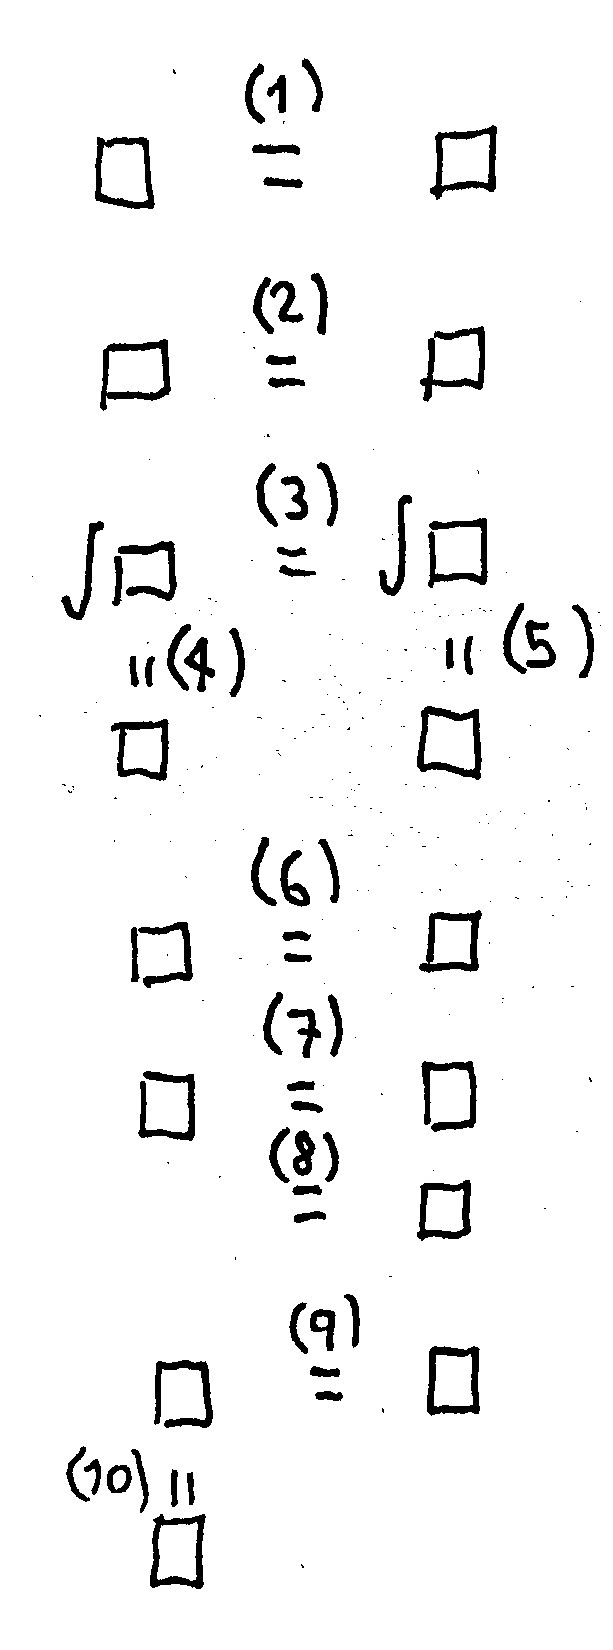
\includegraphics[height=#1]{2021-1-C2/20210916_EDOVSG1_numeracao.pdf}
  }}

Em particular:
%
$$\begin{array}{rclc}
  \pfo{EDOVSG1} &=& \scalebox{0.7}{$\EDOVSGone$}
                  & \left( \numeracao{4.5cm} \right) \\
  \\[-5pt]
  \pfo{EDOVSG2} &=& \scalebox{0.7}{$\EDOVSGtwo$} \\
  \end{array}
$$

\newpage

% «questao-1»  (to ".questao-1")
% (c2m211p2p 4 "questao-1")
% (c2m211p2a    "questao-1")
% (c2m211edovsp 23 "exercicio-6")
% (c2m211edovsa    "exercicio-6")


{\bf Questão 1.}

\T(Total: 5.0 pts)

\ssk


\def\SubstQuestaoUm{
  \bmat{ f(x) := 2x+3 \\
         F(x) := x^2+3x \\
         g(y) := y^4 \\
         G(y) := y^5 + 2 \\
         G^{-1}(x) := \sqrt[5]{x - 2} \\
       }
  }

a) \B(2.0 pts) Escreva o resultado da substituição 
%
$$\pfo{EDOVSG1} \;
  \scalebox{0.8}{$
  \SubstQuestaoUm
  $}
$$

e escreva ``$= \pfo{Q1}$'' à direita do seu resultado

pra indicar que nós vamos usar a expressão $\pfo{Q1}$

pra nos referir a essa expressãozona.

\bsk

Dicas:

{\footnotesize

% (c2m211edovsp 24 "exercicio-6-dica")
% (c2m211edovsa    "exercicio-6-dica")
%    http://angg.twu.net/LATEX/2021-1-C2-edovs.pdf#page=24
\url{http://angg.twu.net/LATEX/2021-1-C2-edovs.pdf#page=24}

% (c2m211substp 9 "igual-depois-de-subst")
% (c2m211substa   "igual-depois-de-subst")
%    http://angg.twu.net/LATEX/2021-1-C2-subst.pdf#page=9
\url{http://angg.twu.net/LATEX/2021-1-C2-subst.pdf#page=9}


}


\newpage

% «questao-1-cont»  (to ".questao-1-cont")
% (c2m211p2p 3 "questao-1-cont")
% (c2m211p2a   "questao-1-cont")

{\bf Questão 1 (cont.)}

Aqui vou usar `(1)', `(2)', ..., `(10)' pra me referir às

igualdades da expressãozona \pfo{Q1} que você definiu no item a.

\msk

b) \B(1.0 pts) Mostre que $y=\sen x$ não é uma solução da EDO
(1).

\ssk

c) \B(0.5 pts) Mostre que (4) é falsa.

\ssk

d) \B(0.5 pts) Mostre que (5) é verdadeira.

\ssk

e) \B(0.5 pts) Digamos que $x=-2$, $y=1$, $C_1=10$.

Encontre o único valor de $C_2$ que faz a (6) ser verdadeira.

\ssk

f) \B(0.5 pts) Mostre que a (10) é verdadeira.

\newpage

% «questao-2»  (to ".questao-2")
% (c2m211p2p 7 "questao-2")
% (c2m211p2a   "questao-2")

{\bf Questão 2.}

\T(Total: 6.0 pts)

\msk

Seja $(*)$ esta EDO daqui:
%
$$\D \frac{dy}{dx} = \frac{x}{y}$$



a) \B(1.0 pts) Desenhe o campo de direções dela. Obs:

Faça tracinhos nos pontos com $x,y∈\{-2,-1,0,1,2\}$.

\ssk

b) \B(1.0 pts) Encontre a solução geral dela e teste-a.

\ssk

c) \B(1.0 pts) Encontre a solução da $(*)$ que passa pelo

ponto $(3,2)$. Diga qual é o domínio dela e teste-a.

\ssk

d) \B(1.0 pts) Encontre a solução da $(*)$ que passa pelo

ponto $(-1,-3)$. Diga qual é o domínio dela e teste-a.

% Dica:
% (c2m202p2p 20 "questao-2-gab")
% (c2m202p2a    "questao-2-gab")
% (c2m202edovsa  "videos")

\newpage

% «questao-2-cont»  (to ".questao-2-cont")
% (c2m211p2p 8 "questao-2-cont")
% (c2m211p2a   "questao-2-cont")

{\bf Questão 2 (cont.)}

\msk

e) \B(0.0 pts) Agora \ColorRed{defina, usando a sintaxe certa,} as

funções $f_b(x)$, $f_c(x)$, $f_d(x)$ que correspondem às funções

que você obteve nos itens b, c e d. Este item vale 0 pontos

\ColorRed{mas se você errar ele todos os próximos itens desta questão

vão ser anulados}.

\bsk

\ColorRed{\bf MUITO IMPORTANTE:} aqui a sua resposta

\ColorRed{\underline{\bf TEM QUE}} começar com um ``sejam'' --- se você

não escrever o ``sejam'' eu vou considerar que

a sua resposta está errada.

\bsk

Obs: na definição da sua $f_b(x)$ você pode usar `$\pm$',

mas nas outros não.


\newpage

{\bf Questão 2 (cont.)}

\msk

f) \B(1.0 pts) Descubra qual é a substituição da forma
%
$$\pfo{EDOVSG2} \;
    \scalebox{0.8}{$
    \bmat{
    f(x) := \Rdq \\
    F(x) := \Rdq \\
    g(y) := \Rdq \\
    G(y) := \Rdq \\
    G^{-1}(x) := \Rdq \\
    C_3 := \Rdq \\
    }
    $}
$$

que resolve a EDO $(*)$ e dá a sua solução $y=f_c(x)$.

Escreva ela por extenso como você fez no item 1a ---

mas note que agora estamos usando a \pfo{EDOVSG2}.

\msk


g) \B(1.0 pts) Faça a mesma coisa para a $y=f_d(x)$.


\newpage

% «gabarito»  (to ".gabarito")
% (c2m211p2p 10 "gabarito")
% (c2m211p2a    "gabarito")

\thispagestyle{empty}

\begin{center}

\vspace*{2.0cm}

{\bf \Large Gabarito}

\end{center}

\newpage

% «questao-1a-gab»  (to ".questao-1a-gab")
% (c2m211p2p 11 "questao-1a-gab")
% (c2m211p2a    "questao-1a-gab")

{\bf Questão 1a}

\sa{f(x)}{f(x)}
\sa{F(x)}{F(x)}
\sa{g(y)}{g(y)}
\sa{G(y)}{G(y)}
\sa{GiGy}{G^{-1}(G(y))}
\sa{GiFx}{G^{-1}(F(x) + C_3)}
\sa{Gix}{foo}

\sa{f(x)}{2x+3}
\sa{F(x)}{x^2 + 3x}
\sa{g(y)}{y^4}
\sa{G(y)}{y^5 + 2}
\sa {Gix}{\sqrt[5]{x - 2}}
\sa{GiGy}{\sqrt[5]{(y^5 + 2) - 2}}
\sa{GiFx}{\sqrt[5]{(x^2 + 3x + C_3) - 2}}

\def\SubstQuestaoUm{
  \bmat{ f(x) := 2x+3 \\
         F(x) := x^2+3x \\
         g(y) := y^4 \\
         G(y) := y^5 + 2 \\
         G^{-1}(x) := \sqrt[5]{x - 2} \\
       }
  }

\def\EDOVSGoneTmp{
  \left(
  \begin{array}{rcl}
  \D \frac{dy}{dx} &=& \D \frac{\ga{f(x)}}{\ga{g(y)}} \\ [10pt]
        \ga{g(y)} \, dy &=&   (\ga{f(x)}) \, dx         \\ [5pt]
      ∫ \ga{g(y)} \, dy &=& ∫ \ga{f(x)} \, dx         \\
        \rotl{=}\ph{mm} & & \ph{mm}\rotl{=}           \\[-5pt]
        \ga{G(y)} + C_1 & & \ga{F(x)} + C_2           \\
                                               [5pt]
        \ga{G(y)} + C_1 &=& \ga{F(x)} + C_2           \\ [5pt]
        \ga{G(y)}       &=& \ga{F(x)} + C_2 - C_1     \\
                        &=& \ga{F(x)} + C_3           \\
                                               [5pt]
              \ga{GiGy} &=& \ga{GiFx}                 \\
        \rotl{=}\ph{mm} & &                           \\[-5pt]
               y\ph{mm} & &                           \\
  \end{array}
  \right)
  }

\def\SubstQuestaoUmTmp{
  \bmat{ f(x) := \ga{f(x)} \\
         F(x) := \ga{F(x)} \\
         g(y) := \ga{g(y)} \\
         G(y) := \ga{G(y)} \\
         G^{-1}(x) := \ga{Gix} \\
       }
  }

$$\scalebox{0.6}{$
    \EDOVSGone
    \SubstQuestaoUmTmp
    =
    \EDOVSGoneTmp
    =
    \pfo{Q1}
  $}
$$

\newpage

% «questoes-1bc-gab»  (to ".questoes-1bc-gab")
% (c2m211p2p 12 "questoes-1bc-gab")
% (c2m211p2a    "questoes-1bc-gab")

{\bf Questões 1b e 1c}

\def\ddy{\frac{d}{dy}}

1b) \qquad
$
  \begin{array}[t]{rcl}
             y & =  & \sen x                  \\
          f(x) & =  & \sen x                  \\
         \dydx &\eqq& \frac{2x+3}{y^4}        \\
   \eqvs{}{ii} &    & \eqvs{m}{}              \\[-5pt]
     \ddx f(x) &    & \frac{2x+3}{(\sen x)^4} \\
    \eqvs{}{m} &    &                         \\[-5pt]
        \cos x &    &                         \\
        \cos x &\neq& \frac{2x+3}{(\sen x)^4} \\
  \end{array}
$

\bsk

1c) \qquad
$
  \begin{array}[t]{rcl}
    \inty{y^4} &\eqq& y^5 + 2 + C_1  \\
          y^4  &\eqq& \ddy(y^5 + 2 + C_1)  \\
               &   =& 5y^4  \\
          y^4  &\neq& 5y^4  \\
    \inty{y^4} &\neq& y^5 + 2 + C_1  \\
  \end{array}
$

\newpage

% «questoes-1def-gab»  (to ".questoes-1def-gab")
% (c2m211p2p 13 "questoes-1def-gab")
% (c2m211p2a    "questoes-1def-gab")

{\bf Questões 1d até 1f}

\msk

1d) \qquad
$
  \begin{array}[t]{rcl}
   \intx{2x+3} &\eqq&      x^2 + 3x + C_2  \\
         2x+3  &\eqq& \ddx(x^2 + 3x + C_2)  \\
               &   =& 2x + 3  \\
   \intx{2x+3} &  = &      x^2 + 3x + C_2  \\
  \end{array}
$

\bsk

1e) A igualdade (6) é $y^5 + 2 + C_1 = x^2 + 3x + C_2$.

Se $x=-2$, $y=1$, $C_1=10$, podemos reescrevê-la

como: $1^5 + 2 + 10 = (-2)^2 + 3(-2) + C_2$; e aí

$C_2 = 1^5 + 2 + 10 - ((-2)^2 + 3(-2)) = 13 - (-2) = 15$.


\bsk

1f) \qquad
$\begin{array}[t]{rcl}
 y &\eqq& \sqrt[5]{(y^5 + 2) - 2} \\
   &   =& \sqrt[5]{y^5} \\
   &   =& y \\
 \end{array}
$

\newpage

% «questoes-2ab-gab»  (to ".questoes-2ab-gab")
% (c2m211p2p 14 "questao-2-gab")
% (c2m211p2a    "questao-2-gab")

{\bf Questões 2a e 2b}


% (find-latexscan-links "C2" "20210920_gab_1b")
% (find-xpdf-page "~/LATEX/2021-1-C2/20210920_gab_1b.pdf")
%\includegraphics[height=8cm]{2021-1-C2/20210920_gab_1b.pdf}

2a) \quad
% (find-latexscan-links "C2" "20210920_gab_2a")
% (find-xpdf-page "~/LATEX/2021-1-C2/20210920_gab_2a.pdf")
$\myvcenter{
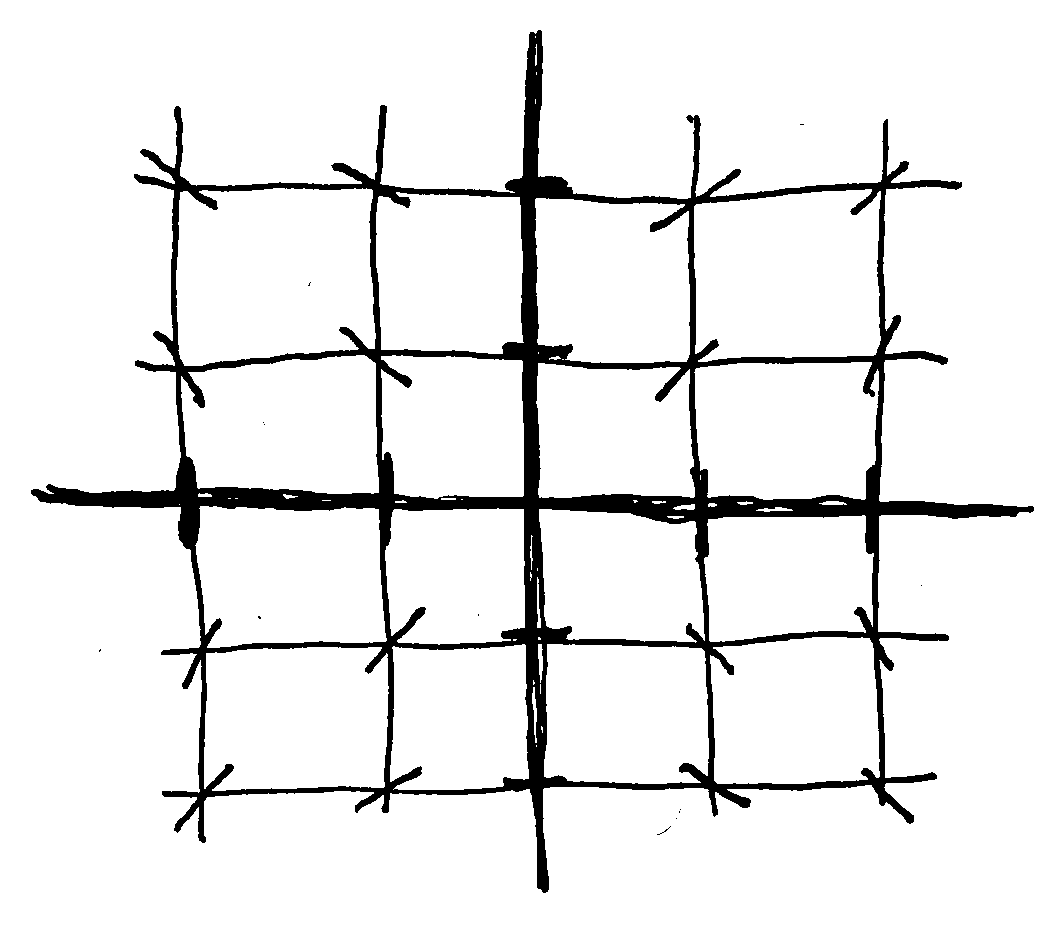
\includegraphics[height=3cm]{2021-1-C2/20210920_gab_2a.pdf}
}$
%
\qquad
%
2b) \quad
% (find-latexscan-links "C2" "20210920_gab_2b")
% (find-xpdf-page "~/LATEX/2021-1-C2/20210920_gab_2b.pdf")
$\myvcenter{
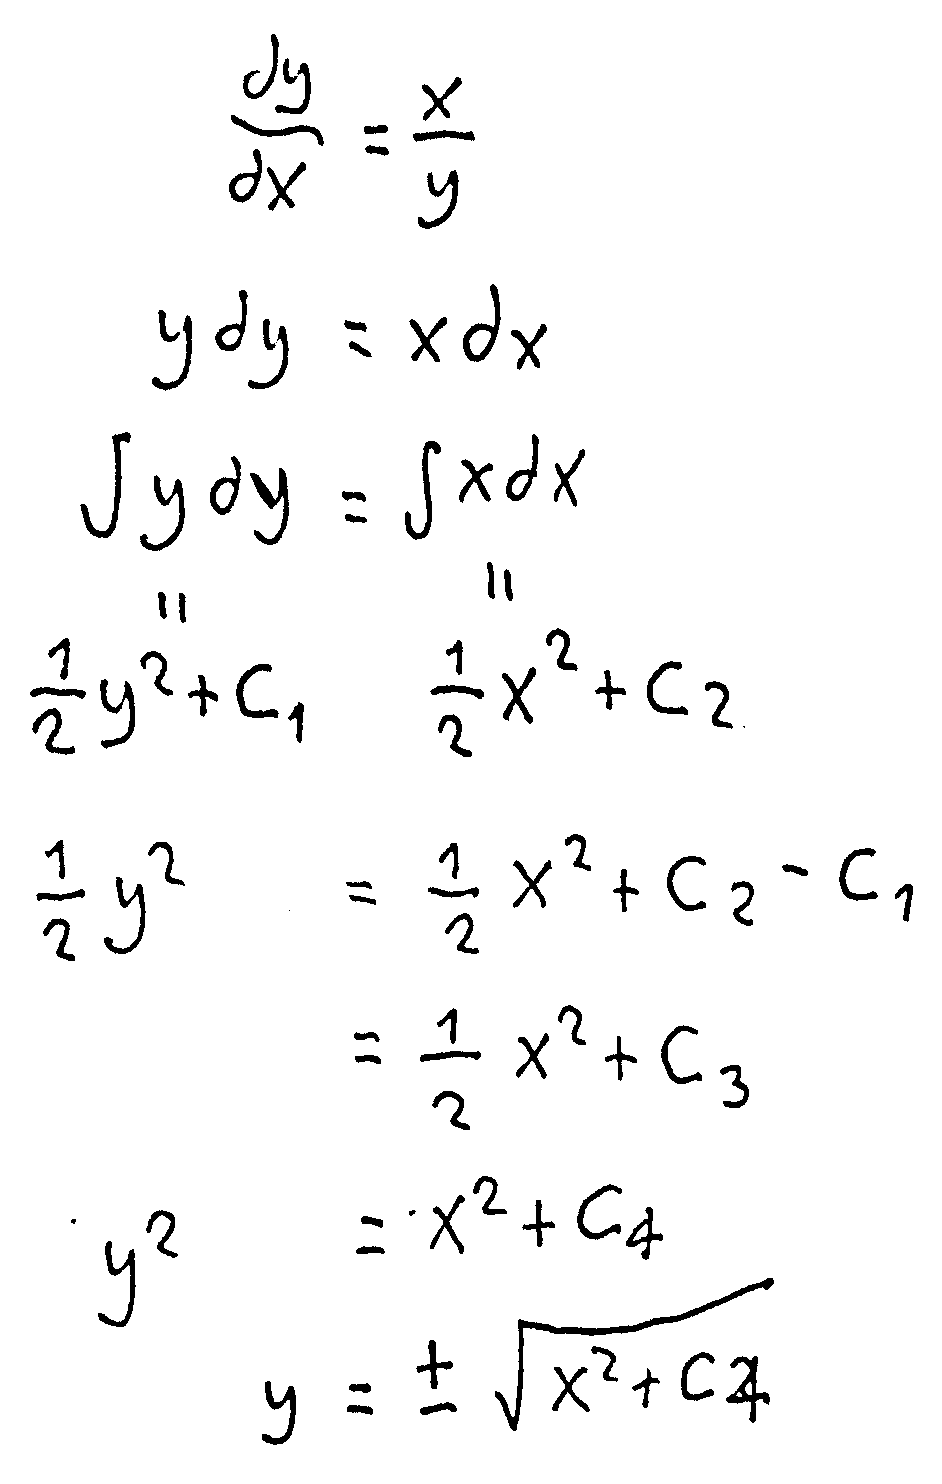
\includegraphics[height=5cm]{2021-1-C2/20210920_gab_2b.pdf}
}$

(Falta o teste da 2b)

\newpage

% «questoes-2cd-gab»  (to ".questoes-2cd-gab")
% (c2m211p2p 15 "questoes-2cd-gab")
% (c2m211p2a    "questoes-2cd-gab")

{\bf Questões 2c e 2d}

\msk

2c)
\quad
%
% (find-latexscan-links "C2" "20210920_gab_2c")
% (find-xpdf-page "~/LATEX/2021-1-C2/20210920_gab_2c.pdf")
$\myvcenter{
 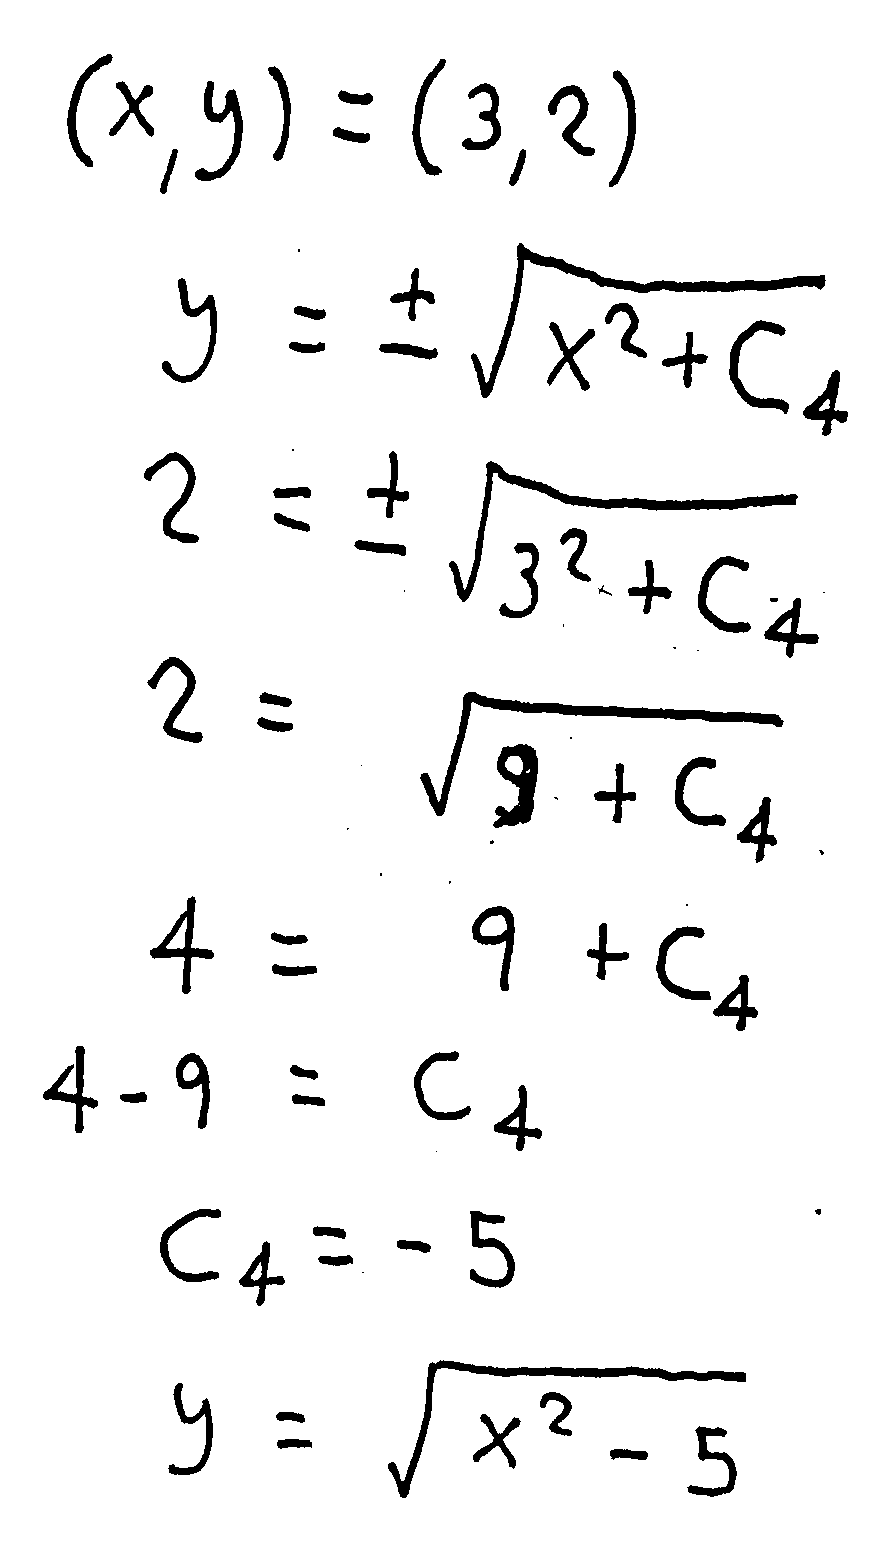
\includegraphics[height=3cm]{2021-1-C2/20210920_gab_2c.pdf}
}$
%
\quad
%
$\begin{array}{l}
 \text{Domínio:} \\
  \setofst{x∈\R}{x^2 - 5 ≥ 0} \\
  = \;\; \setofst{x∈\R}{x^2 ≥ 5} \\
  = \;\; \setofst{x∈\R}{|x| ≥ \sqrt{5}} \\
  = \;\; (-∞,\sqrt{5}] ∪ [\sqrt{5},+∞) \\
 \end{array}
$

(Falta o teste)

\bsk


2d)
%
$
% (find-latexscan-links "C2" "20210920_2d_solucao")
% (find-xpdf-page "~/LATEX/2021-1-C2/20210920_2d_solucao.pdf")
\myvcenter{
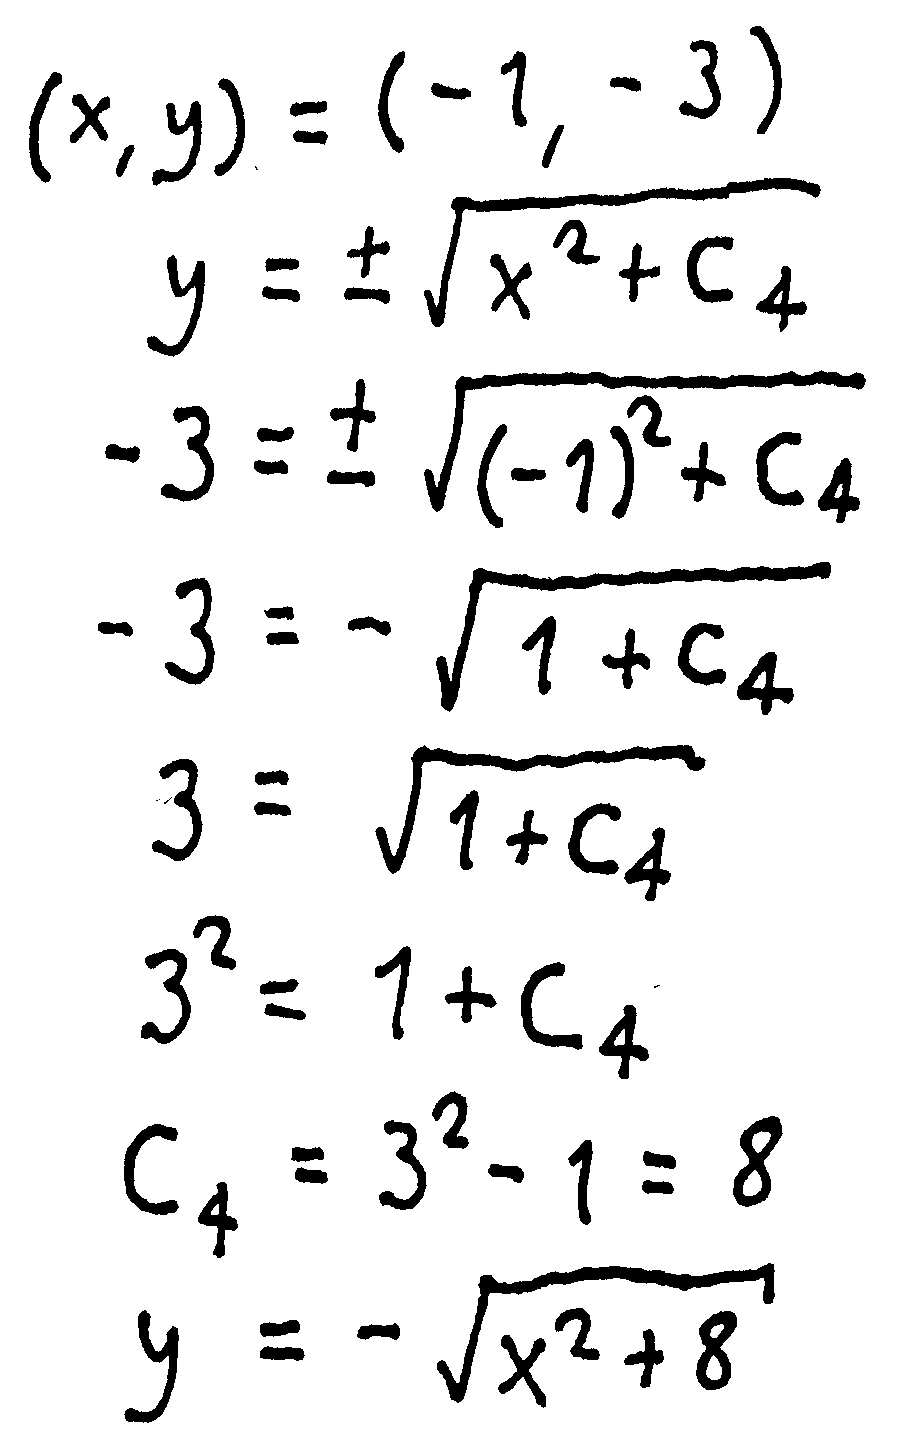
\includegraphics[height=3cm]{2021-1-C2/20210920_2d_solucao.pdf}
}
%
\quad
%
\begin{array}{c}
% (find-latexscan-links "C2" "20210920_2d_dominio")
% (find-xpdf-page "~/LATEX/2021-1-C2/20210920_2d_dominio.pdf")
\myvcenter{
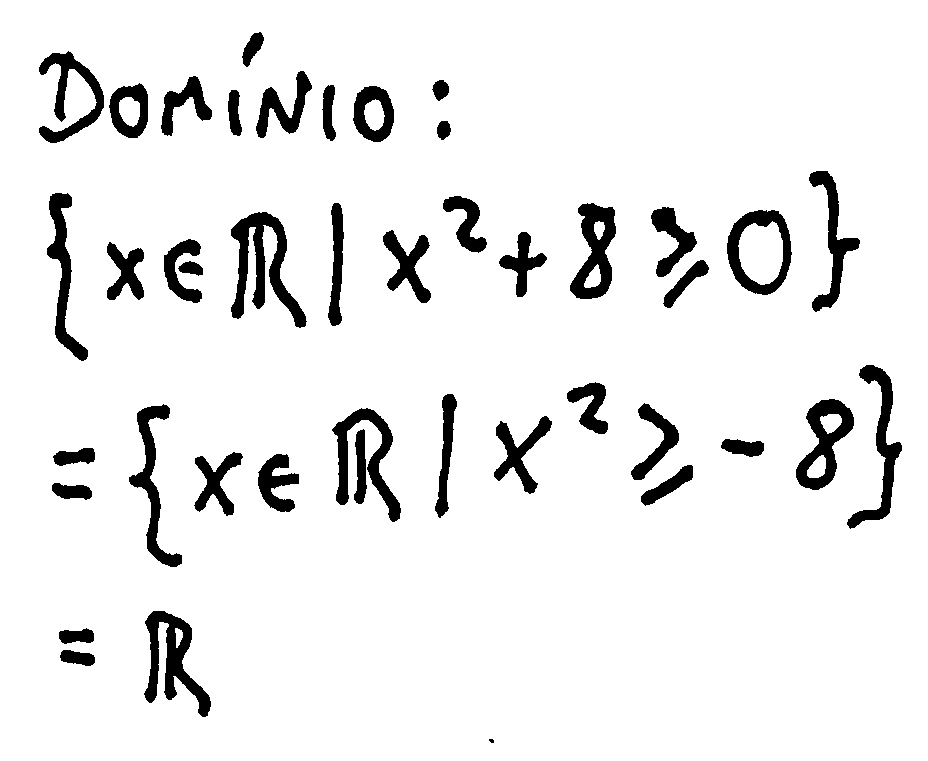
\includegraphics[height=1.5cm]{2021-1-C2/20210920_2d_dominio.pdf}
}
%
\quad
%
% (find-latexscan-links "C2" "20210920_2d_teste")
% (find-xpdf-page "~/LATEX/2021-1-C2/20210920_2d_teste.pdf")
\myvcenter{
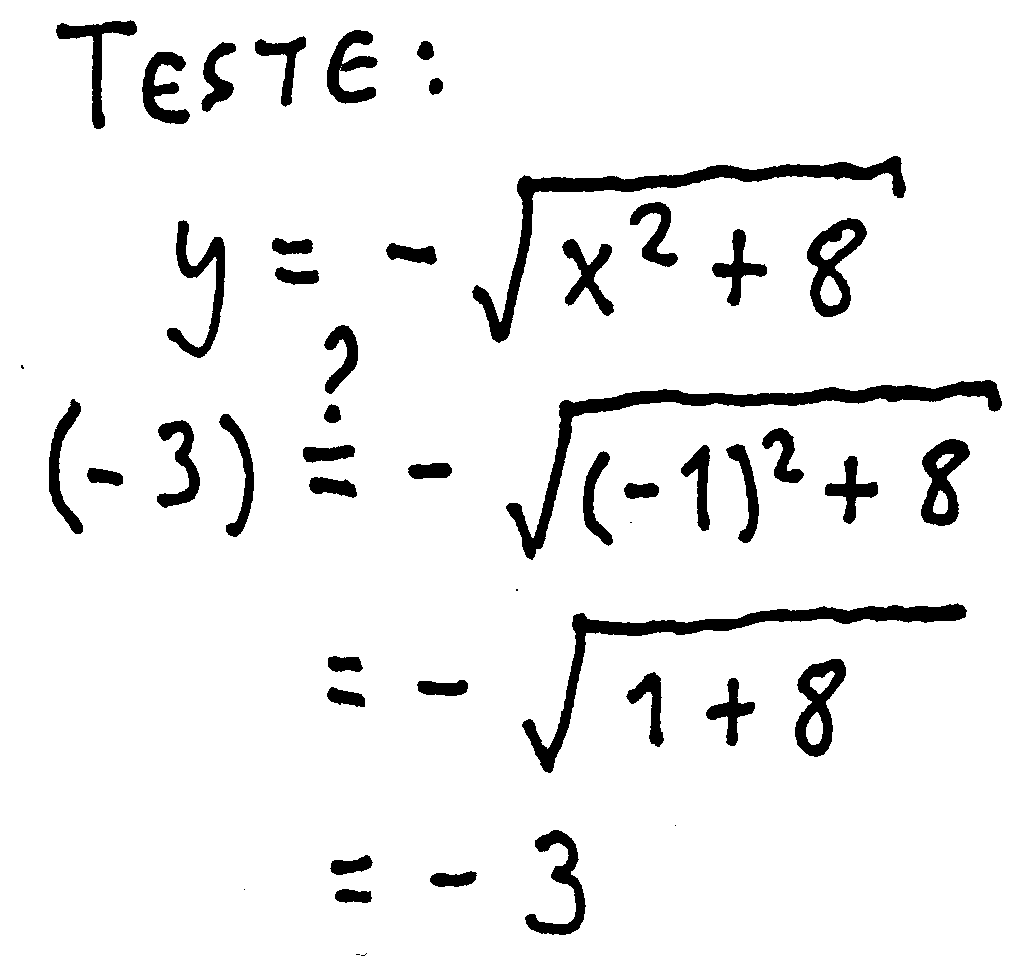
\includegraphics[height=2.0cm]{2021-1-C2/20210920_2d_teste.pdf}
}
\end{array}
$






\newpage

% «questao-2e-gab»  (to ".questao-2e-gab")
% (c2m211p2p 16 "questao-2e-gab")
% (c2m211p2a    "questao-2e-gab")

{\bf Questão 2e}

\msk

2e) Sejam:
%
$\begin{array}[t]{rcl}
 f_b(x) &=& \pm \sqrt{x^2 + C_4}, \\
 f_c(x) &=&     \sqrt{x^2 - 5}, \\
 f_d(x) &=&  -  \sqrt{x^2 + 8}. \\
 \end{array}
$

\bsk
\bsk
\bsk

Truque pra 2f e pra 2g:

Lembre que na 2b nós fizemos essa passagem aqui:
%
$$\begin{array}{rcl}
  \frac12 y^2 &=& \frac12 x^2 + C_3 \\
          y^2 &=& x^2 + C_4 \\
  \end{array}
$$

Nela ficava implícito que $2C_3 = C_4$.


\newpage

% «questoes-2fg-gab»  (to ".questoes-2fg-gab")
% (c2m211p2p 17 "questoes-2fg-gab")
% (c2m211p2a    "questoes-2fg-gab")

\bsk


2f) Para $f_b(x) = \pm \sqrt{x^2 + C_4}$:

\ph{2f)} (Ou: $f_b(x) = \pm \sqrt{x^2 + 2C_3}$ ...)
%
\def\SubstQuestaoUmTmp{
  \bmat{ f(x) := x \\
         F(x) := \frac12 x^2 \\
         g(y) := y \\
         G(y) := \frac12 y^2 \\
         G^{-1}(x) := \pm \sqrt{2x} \\
         C_3 := \frac12 C_4 \\
       }
  }
\def\EDOVSGtwoTmp{
  \left(
  \begin{array}{rcl}
  \D \frac{dy}{dx} &=& \D \frac{x}{y} \\ [10pt]
                 y &=& \pm \sqrt{2(\frac12 x^2 + \frac12 C_4)}   \\
  \end{array}
  \right)
  }
%
$$\scalebox{0.7}{$
    \EDOVSGtwo
    \SubstQuestaoUmTmp
    =
    \EDOVSGtwoTmp
  $}
$$

\bsk
\bsk


2g) Para $f_c(x) = \sqrt{x^2 - 5}$:
%
\def\SubstQuestaoUmTmp{
  \bmat{ f(x) := x \\
         F(x) := \frac12 x^2 \\
         g(y) := y \\
         G(y) := \frac12 y^2 \\
         G^{-1}(x) := \sqrt{2x} \\
         C_3 := - \frac52 \\
       }
  }
\def\EDOVSGtwoTmp{
  \left(
  \begin{array}{rcl}
  \D \frac{dy}{dx} &=& \D \frac{x}{y} \\ [10pt]
                 y &=& \sqrt{2(\frac12 x^2 + (-\frac52))}   \\
  \end{array}
  \right)
  }
%
$$\scalebox{0.7}{$
    \EDOVSGtwo
    \SubstQuestaoUmTmp
    =
    \EDOVSGtwoTmp
  $}
$$






%\printbibliography

\GenericWarning{Success:}{Success!!!}  % Used by `M-x cv'

\end{document}

%  ____  _             _         
% |  _ \(_)_   ___   _(_)_______ 
% | | | | \ \ / / | | | |_  / _ \
% | |_| | |\ V /| |_| | |/ /  __/
% |____// | \_/  \__,_|_/___\___|
%     |__/                       
%
% «djvuize»  (to ".djvuize")
% (find-LATEXgrep "grep --color -nH --null -e djvuize 2020-1*.tex")

 (eepitch-shell)
 (eepitch-kill)
 (eepitch-shell)
# (find-fline "~/2021.1-C2/")
# (find-fline "~/LATEX/2021-1-C2/")
# (find-fline "~/bin/djvuize")

cd /tmp/
for i in *.jpg; do echo f $(basename $i .jpg); done

f () { rm -v $1.pdf;  textcleaner -f 50 -o  5 $1.jpg $1.png; djvuize $1.pdf; xpdf $1.pdf }
f () { rm -v $1.pdf;  textcleaner -f 50 -o 10 $1.jpg $1.png; djvuize $1.pdf; xpdf $1.pdf }
f () { rm -v $1.pdf;  textcleaner -f 50 -o 20 $1.jpg $1.png; djvuize $1.pdf; xpdf $1.pdf }

f () { rm -fv $1.png $1.pdf; djvuize $1.pdf }
f () { rm -fv $1.png $1.pdf; djvuize WHITEBOARDOPTS="-m 1.0 -f 15" $1.pdf; xpdf $1.pdf }
f () { rm -fv $1.png $1.pdf; djvuize WHITEBOARDOPTS="-m 1.0 -f 30" $1.pdf; xpdf $1.pdf }
f () { rm -fv $1.png $1.pdf; djvuize WHITEBOARDOPTS="-m 1.0 -f 45" $1.pdf; xpdf $1.pdf }
f () { rm -fv $1.png $1.pdf; djvuize WHITEBOARDOPTS="-m 1.0 -f 75" $1.pdf; xpdf $1.pdf }
f () { rm -fv $1.png $1.pdf; djvuize WHITEBOARDOPTS="-m 0.5" $1.pdf; xpdf $1.pdf }
f () { rm -fv $1.png $1.pdf; djvuize WHITEBOARDOPTS="-m 0.25" $1.pdf; xpdf $1.pdf }
f () { cp -fv $1.png $1.pdf       ~/2021.1-C2/
       cp -fv        $1.pdf ~/LATEX/2021-1-C2/
       cat <<%%%
% (find-latexscan-links "C2" "$1")
%%%
}

f 20210920_2d_dominio
f 20210920_2d_solucao
f 20210920_2d_teste




%  __  __       _        
% |  \/  | __ _| | _____ 
% | |\/| |/ _` | |/ / _ \
% | |  | | (_| |   <  __/
% |_|  |_|\__,_|_|\_\___|
%                        
% <make>

 (eepitch-shell)
 (eepitch-kill)
 (eepitch-shell)
# (find-LATEXfile "2019planar-has-1.mk")
make -f 2019.mk STEM=2021-1-C2-P2 veryclean
make -f 2019.mk STEM=2021-1-C2-P2 pdf

% Local Variables:
% coding: utf-8-unix
% ee-tla: "c2p2"
% ee-tla: "c2m211p2"
% End:
